\section{The microtubule}
We've already mentioned that cells employ motor proteins and the cytoskeleton to solve the cellular transport problem. The following figure demonstrates the complexity of this network of cellular highways within endothelial cells. 
\begin{figure}[!hbt]
	\centering
	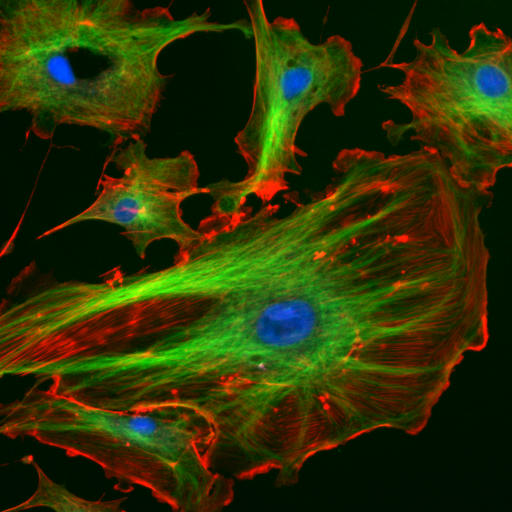
\includegraphics[width=0.5\columnwidth]{cytoskeleton}
	\caption{Endothelial cells with their cytoskeleton structures shown. The nucleus of each cell is colored in blue. Actin filaments are shown in red and tubulin is shown in green. Image taken from \cite{cytoskeleton}}
	\label{fig:cytoskeleton}
\end{figure}

Dynein walks along a particular cyctoskeleton filament called a microtubule. Microtubules are cytoskeletal structures formed by self assembly of $\alpha$ and $\beta$ tubulin heterodimers (shown as green in Figure \ref{fig:cytoskeleton}). \cite{downing_tubulin_1998} These molecular structures are typically comprised of 13 protofilaments each of which is a periodic arrangement of the $\alpha$ and $\beta$ dimers. 

Microtubules exhibit an inherent polarity identified as the plus ($+$) and minus ($-$) ends \cite{lodish_microtubule_2000}. This polarity is both function and structural. One end of the microtubule experiences much faster addition of tubulin making it easy to identify\cite{heidemann_visualization_1980}. For our purposes though, the structural polarity of the microtubule is more important as the formation of the microtubule results in a helical structure that has definite chirality \cite{microtubule_chirality}. Two possible microtubule configurations are shown in Figure \ref{fig:chirality}. Note that even though there is a deviation by angle $\theta$ between the two microtubules, the overall handedness of the helix is the same. 

\begin{figure}[!hbt]
	\centering 
	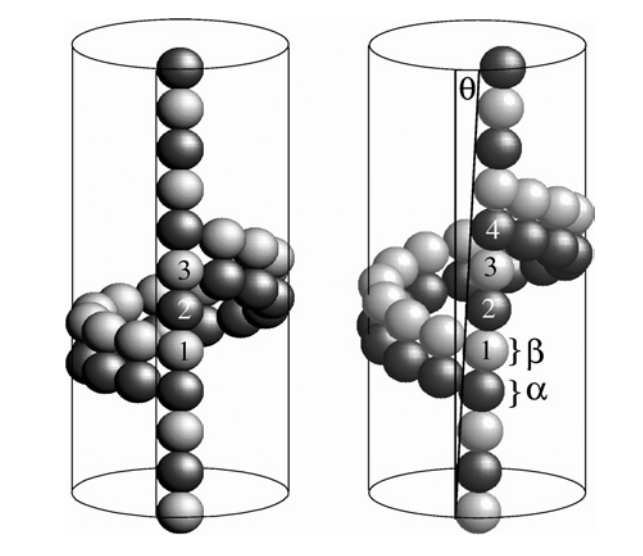
\includegraphics[width=.5\columnwidth]{microtubule_chirality}
	\caption{Two possible microtubule structures illustrating the chirality of the helix as well as the skew angle of the dimers of which only one is shown for illustrative purposes. Image taken from \cite{microtubule_chirality}.}
	\label{fig:chirality}
\end{figure}

As Figure \ref{fig:cytoskeleton} shows, microtubules foliate the entire cell with paths that enable motor proteins to move cargo. Most(not all) variations of the kinesin molecular motor are plus-end directed. They are almost always observed to walk towards the plus-end of the microtubule. Dynein is strictly a minus-end directed motor \cite{alberts_molecular_2002}. How this directed motion is derived from the symmetric dynein structure is still an open question.\\



\section{The powerstroke model} 
Take another look at Figure \ref{fig:motor proteins}. How does this complicated structure perform complex locomotion using only the resources of its aqueous environment? How can a highly symmetric structure lead to directed motion? The chemical resolution to this problem arises from the interaction of ATP with each of the motor domains of dynein. The cycle of converting the chemical energy of  ATP into useful mechanical energy for motion is called the \textit{mechanochemical cycle}\cite{cianfrocco_mechanism_2015}. Describing all of the chemical interactions involved in a single dynein step has been an active area of research. The currently accepted model was proposed by Cianfrocco et al. and is summarized in the following graphic shown in Figure \ref{fig:mechanochemical_cycle}. 

\begin{figure}[!hbt]
	\centering
	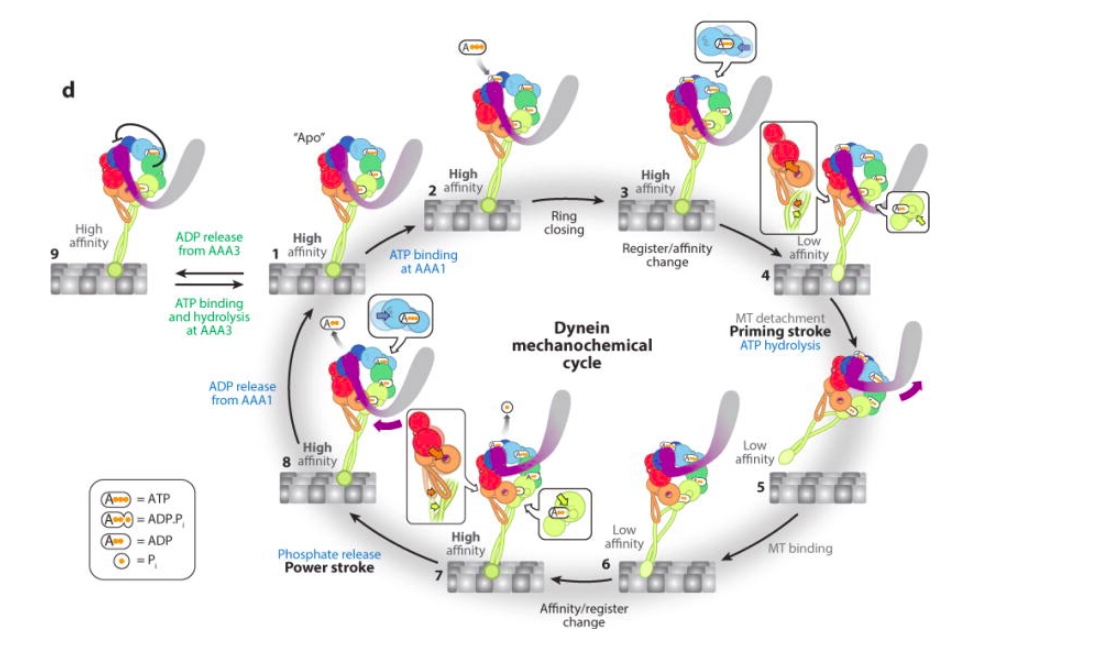
\includegraphics[width=1\columnwidth]{mechanochemical_cycle}
	\caption{The mechanochemical cycle of dynein. Dynein goes through many identifiable stages as ATP from the environment interacts with the motor domain and changes the conformation of the protein. Image taken from \cite{cianfrocco_mechanism_2015}.}
	\label{fig:mechanochemical_cycle}
\end{figure}

The important takeaway from Figure \ref{fig:mechanochemical_cycle} is that we can identify a ``pre-stroke" and a ``post-stroke" state corresponding to the conformational change that occurs in the purple linker between steps 7 and 8. These states are again illustrated in the following figure to make the physical change in shape clear. 

\begin{figure}[!hbt]
	\centering
	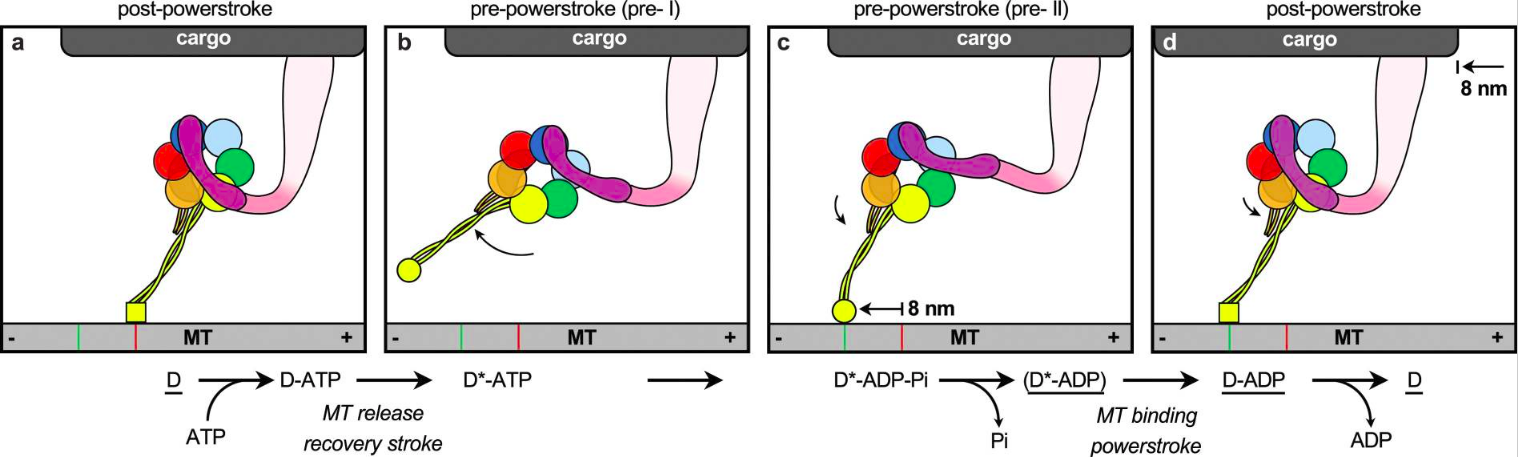
\includegraphics[width=1\columnwidth]{pre_post_powerstroke}
	\caption{An illustration of the pre and post stroke states of dynein in relation to the microtubule and the cargo that they carry. This two-dimensional illustration shows only one of legs of dynein. Image taken from \cite{dynein_powerstroke}.}
\end{figure}

Scientists have determined the steps of this chemical cycle by carefully isolating and analyzing the resulting structures via cryo-electron microscopy \cite{cryo_em}. While this is useful for determining the conformation before and after a chemical process occurs, it does note describe the actual motion along the microtubule-- only intermittent states. All of the information about how flexible each domain is during binding and to what extent the protein diffuses in its search for the microtubule require alternative methods to establish.

\section{Other observational techniques} 
 Kinesin and Dynein have masses of a few hundred kDa and  $\sim2$ MDa respectively \cite{liao_kinesin_1998, johnson_structure_1983}. Recalling that 1 Dalton (Da) corresponds to one atomic mass unit means these proteins consist of, at most, a few million atoms. This small scale poses a unique experimental challenge. One way this is approached at Prof. Weihong Qiu's group is by attaching small fluorescent molecules called fluorophores to the binding sites that motor proteins use to latch onto their cargo. Then, the individual movement of motors can be tracked using total internal reflection fluorescence microscopy to produce video of the proteins in action as illustrated in figure \ref{fig:weihong tirf} from \cite{qiu_dynein_2012}. 

\begin{figure}[!hbt]
	\centering
	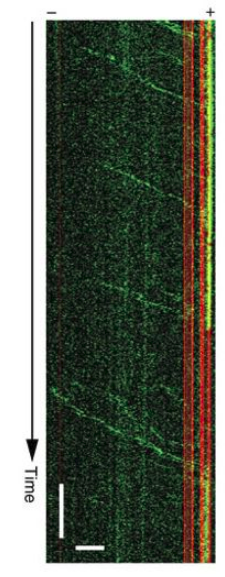
\includegraphics[angle=90, width=0.75\columnwidth]{weihong_motor}
	\caption{\textbf{TIRF Microscopy Imaging} individual kinesin proteins are imaged as small green dots and tracked as they move. Slices at different times are stacked so that the slope of each green line indicates the velocity of the protein. Image taken from \cite{qiu_dynein_2012}.}
	\label{fig:weihong tirf}
\end{figure}

Figure \ref{fig:weihong tirf} demonstrates fluorescence microscopy enables observation of protein speed, how far it walks along the microtubule, which direction is preferred. Furthermore, by tagging a motor domain instead of the tail, this technique can resolve step sizes and as shown in Figure \ref{fig:weihong histogram}. \cite{qiu_dynein_2012} Taking into account these studies as well as the delicate cryo-em analysis forms a rough sketch for dynein's motion. Unfortunately though, this is the limit of current experimental methods; observing the individual motions of each of the binding domains of a dynein protein is not yet possible. 


\todo[inline]{TODO: Add in discussion of using gold particles + scattering to observe Brownian wiggling. This was a result of conversations with Colloquium speaker Kazuhiro Oiwa.}

\section{Experimental stepping statistics}
Here I will include the various stepping statistics (distribution, binding/unbinding rates, etc...) that we hope to fit our simulation to.


\section{More motivation} 
Here I will discuss other simulation efforts that, in our opinion, make far to many assumptions or are purely monte carlo and don't actually simulate the motion of the protein. I will also discuss why our simulation is a happy medium between a full on molecular dynamics simulation (time expensive but accurate) and monte carlo (very fast but doesn't dynamically simulate the protein and instead just selects steps from a distribution). 